\subsection{Jednoduchá $\delta$ jáma nebo bariéra}
\label{sec:Delta}
Částice o hmotnosti $M$ se nachází v potenciálu ve tvaru jednoduché $\delta$ funkce\index{funkce!delta},
\begin{equation}
	V(x)=c\,\delta(x),
\end{equation} 
kde $c$ je konstanta, jejíž velikost udává \uv{sílu} potenciálu.
Pokud je $c<0$, jedná se o jámu, v opačném případě o bariéru.

\begin{enumerate}
\item 
    Napište Schrödingerovu rovnici pro tento model a nalezněte podmínky, které musí splňovat vlnová funkce v bodě, ve kterém se nachází $\delta$ funkce.

\item 
    Pro případ jámy $c<0$ nalezněte všechny vázané stavy (tj. stavy se zápornou energií, existují-li) a příslušné normalizované vlastní funkce.

\item 
    Nalezněte řešení pro $E>0$ (v této oblasti je spektrum spojité).
    Vypočítejte pravděpodobnost průchodu $T$ a pravděpodobnost odrazu $R$ na potenciálu a nakreslete graf $T=T(E)$, $R=R(E)$.

\item 
    Vypočítejte fázové posunutí $\delta$ vlnové funkce a zakreslete funkci $\delta=\delta(E)$.
\end{enumerate}

\begin{solution}
	\begin{enumerate}
	\item
		Schrödingerova rovnice\index{rovice!Schrödingerova} pro vlnovou funkci $\psi(x)$ zní 
		\begin{equation}
			\label{eq:DeltaSchrodinger}
            \left[-\frac{\hbar^{2}}{2M}\derivative[2]{}{x}+c\,\delta(x)\right]\psi(x)
                =E\psi(x).
		\end{equation}
		Integrace v malém okolí $x=0$, ve kterém sedí $\delta$ funkce, vede na vztah
		\begin{equation}
			-\frac{\hbar^{2}}{2M}\left[\psi'(\epsilon)-\psi'(-\epsilon)\right]+c\psi(0)
				=E\int_{-\epsilon}^{\epsilon}\psi(x)\d x,
		\end{equation}
		kde $\psi'(x)\equiv\d\psi(x)/\d x$.
		Limita $\epsilon\rightarrow0+$ dá sešívací podmínku\sfootnote{
			Rovnice~\eqref{eq:SewDerivativeDelta} lze též formálně přepsat pomocí logaritmické derivace\index{derivace!logaritmická}
			\begin{equation}
                L(x)\equiv\frac{\psi'(x)}{\psi(x)}
                    =\derivative{}{x}\ln{\psi(x)}
			\end{equation}
			na tvar
			\begin{equation}
				L(0+)-L(0-)=K.
			\end{equation}
		}\index{podmínka!sešívací}
		\begin{equation}
			\label{eq:SewDerivativeDelta}
			\boxed{\psi'(0+)-\psi'(0-)=K\psi(0)},
		\end{equation}
		kde $\psi'(0\pm)$ označuje limitu zleva ($-$), resp. zprava ($+$) funkce $\psi'(x)$ v bodě $x=0$ a
		\begin{equation}\label{eq:DeltaK}
			K=\frac{2Mc}{\hbar^{2}}.
		\end{equation}
        
        \trick{Vlnová funkce při průchodu $\delta$ funkcí potenciálu musí být spojitá a její derivace má skok daný vzorcem~\eqref{eq:SewDerivativeDelta}.}\index{podmínka!sešívací}
		
	\item
		Vázaný stav se musí nacházet na energii $E<0$.
		Pro $x\neq0$ má Schrödingerova rovnice~\eqref{eq:DeltaSchrodinger} tvar jako pro volnou částici
		\begin{equation}
            -\frac{\hbar^{2}}{2M}\derivative[2]{\psi(x)}{x}
                =E\psi(x)
		\end{equation}
		a její obecné řešení je
		\begin{equation}
            \psi(x)
                =A\e^{\kappa x}+B\e^{-\kappa x},
		\end{equation}
		kde $A,B\in\mathbb{C}$ jsou konstanty a
		\begin{equation}
			\label{eq:kappa}
			\kappa=\sqrt{-\frac{2ME}{\hbar^{2}}}.
		\end{equation}
		
		Vlnová funkce v oblastech I (nalevo od $\delta$ funkce, $x<0$) a II (napravo od $\delta$ funkce, $x>0$), viz obrázek~\ref{fig:DeltaWF}, je
		\begin{subequations}
			\begin{align}
				\psi_{\ti{I}}(x)&=A\e^{\kappa x}+B\e^{-\kappa x},  & x&<0,\\
				\psi_{\ti{II}}(x)&=C\e^{\kappa x}+D\e^{-\kappa x}, & x&>0.
			\end{align}
			\label{eq:DeltaWF}				
		\end{subequations}
		Aby byla vlnová funkce normovatelná (kvadraticky integrovatelná), musí vymizet v nekonečnu, $\lim_{x\rightarrow\pm\infty}\psi(x)=0$, z čehož plyne, že
		\begin{equation}
			B=C=0.
		\end{equation}
		Sešívací podmínky [spojitost, skok v derivaci~\eqref{eq:SewDerivativeDelta}] v bodě $x=0$ dávají
		\begin{subequations}
			\begin{align}
				\psi_{\ti{I}}(0)
					&=\psi_{\ti{II}}(0),\\
				\psi'_{\ti{II}}(0)-\psi'_{\ti{I}}(0)
					&=K\psi_{\ti{I}}(0),
			\end{align}
		\end{subequations}
		takže
		\begin{subequations}			
			\begin{align}
				A&=D,\\
				\kappa&=-\frac{K}{2}.
				\label{eq:Deltakappa}
			\end{align}
		\end{subequations}
		Dosazení~\eqref{eq:DeltaK} a~\eqref{eq:kappa} vede na kvantovací podmínku
		\begin{equation}
			\label{eq:DeltaEnergy}
			\boxed{E=-\frac{Mc^{2}}{2\hbar^{2}}},
		\end{equation}
		která udává energii \emph{jediného} vázaného stavu systému.\index{stav!vázaný}
		
		\begin{figure}[!htbp]
			\centering
			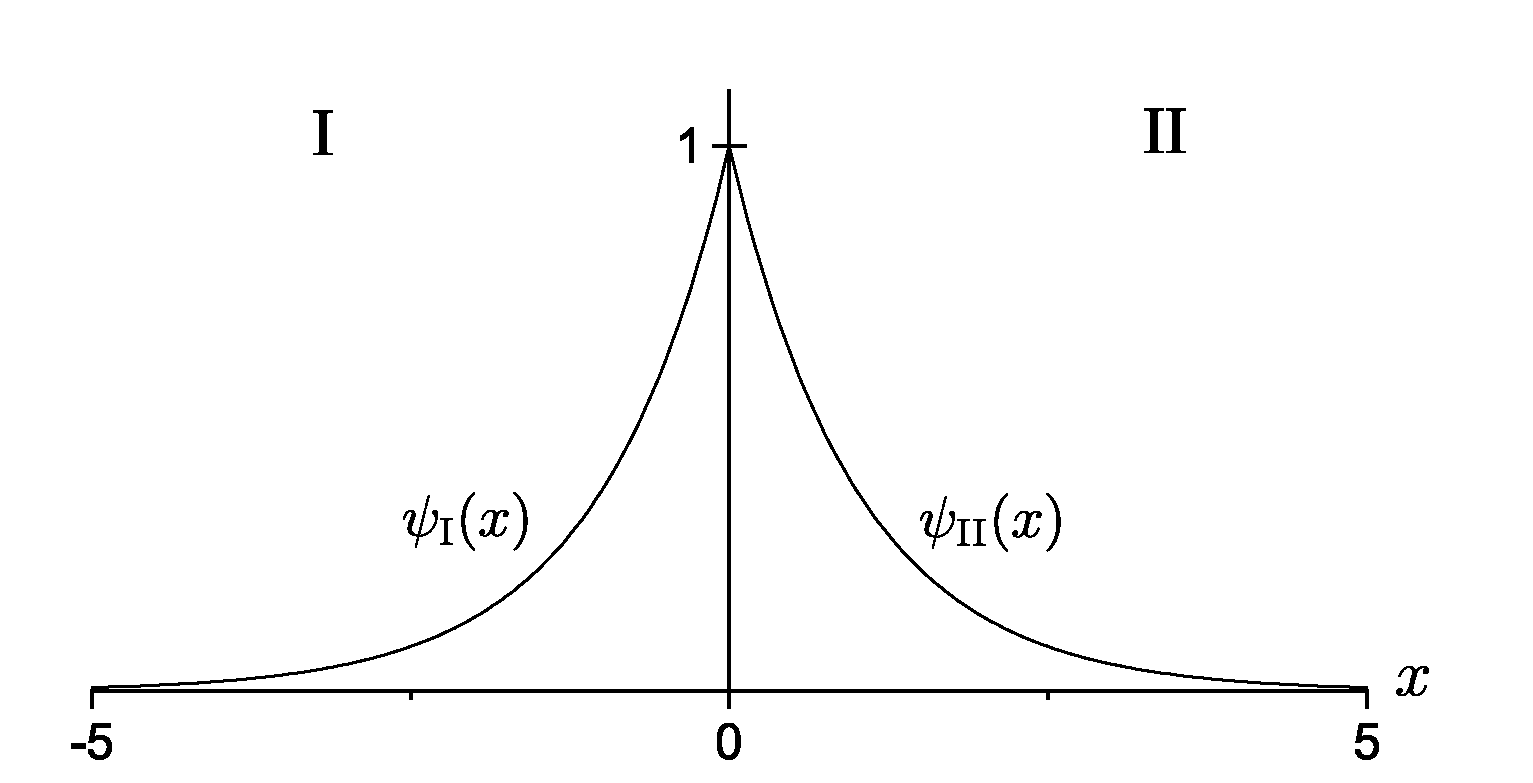
\epsfig{file=figures/deltapsi.eps,width=0.6\linewidth}
			\scaption{
				Normalizovaná vlnová funkce vázaného stavu pro $M=\hbar=1$, $c=-1$.
			}
			\label{fig:DeltaWF}
		\end{figure}
		
		Zbývá nanormovat vlnovou funkci, tj. nalézt hodnotu parametru $A$:
		\begin{align}
			1
			&=\int_{-\infty}^{\infty}\abs{\psi(x)}^{2}\d x
			 =\int_{-\infty}^{0}\abs{\psi_{\ti{I}}(x)}^{2}\d x
				+\int_{0}^{\infty}\abs{\psi_{\ti{II}}(x)}^{2}\d x\nonumber\\
			&=\abs{A}^{2}\left\{\int_{-\infty}^{0}\e^{2\kappa x}\d x
				+\int_{0}^{\infty}\e^{-2\kappa x}\d x\right\}\nonumber\\
			&=\abs{A}^{2}\left\{\left[\frac{1}{2\kappa}\e^{2\kappa x}\right]_{-\infty}^{0}
				+\left[-\frac{1}{2\kappa}\e^{-2\kappa x}\right]_{0}^{\infty}\right\}
			 =\frac{\abs{A}^{2}}{\kappa},
		\end{align}
		Při volbě nulové komplexní fáze normalizačního parametru je
		\begin{equation}
            A=D=\sqrt{\kappa}
                =\sqrt{-\frac{Mc}{\hbar^{2}}}
		\end{equation}
		[veličina $\kappa$ byla vyjádřena pomocí~\eqref{eq:Deltakappa} a~\eqref{eq:kappa}].
		Normalizovaná vlnová funkce vázaného stavu~\eqref{eq:DeltaEnergy} je tedy
		\begin{subequations}
			\begin{align}
				\psi_{\ti{I}}(x)
					&=\sqrt{-\frac{Mc}{\hbar^{2}}}\e^{-\frac{Mc}{\hbar^{2}} x},\\
				\psi_{\ti{II}}(x)
					&=\sqrt{-\frac{Mc}{\hbar^{2}}}\e^{\frac{Mc}{\hbar^{2}} x},
			\end{align}
		\end{subequations}
		nebo souhrnně
		\begin{equation}
			\psi(x)=\sqrt{-\frac{Mc}{\hbar^{2}}}\e^{-\frac{Mc}{\hbar^2}\abs{x}}.
		\end{equation}
		Její průběh je znázorněn na obrázku~\ref{fig:DeltaWF}.
		
	\item
		Jedná se o rozptylovou úlohu na 1D potenciálu.
		Částice přichází z oblasti, ve které je asymptoticky volná, do lokalizované interakční oblasti.
		Interakce způsobí, že se částice může s určitou nenulovou pravděpodobností odrazit. 
		Pokud naopak projde, může se změnit její fáze.
		Tyto změny udávají měřitelné veličiny pravděpodobnost průchodu $T$, pravděpodobnost odrazu $R$ a fázový posun $\delta$.

		V kladných energiích má systém spojité spektrum.
		V oblastech I a II je řešením Schödingerovy rovnice~\eqref{eq:DeltaWF} se vlnová funkce vyjádří jako
		\begin{subequations}
			\begin{align}
				\psi_{\ti{I}}(x)&=A\e^{\im k x}+B\e^{-\im k x},\nonumber\\
				\psi_{\ti{II}}(x)&=C\e^{\im k x}+D\e^{-\im k x},
			\end{align}
			\label{eq:DeltaBarrierWF}
		\end{subequations}
		kde
		\begin{equation}
			k=\sqrt{\frac{2ME}{\hbar^{2}}}.
			\label{eq:k}
		\end{equation}
		
		Pro určení pravděpodobností průchodu\index{pravděpodobnost!průchodu} a odrazu\index{pravděpodobnost!odrazu} se předpokládá, že k $\delta$ funkci přichází vlna zleva (člen úměrný $A$) a rozdělí se na odraženou vlnu (člen úměrný $B$) a prošlou vlnu (člen úměrný $D$).
		Zprava žádná vlna nepřichází, takže $D=0$.
		Hledané pravděpodobnosti se pak definují jako
		\begin{subequations}
			\begin{align}
				R&=\abs{\mathfrak{R}}^{2},
				&\mathfrak{R}&=\frac{B}{A},\\
				T&=\abs{\mathfrak{T}}^{2},
				&\mathfrak{T}&=\frac{C}{A}=\abs{T}\e^{\im\delta},
				\label{eq:PhaseShift}
			\end{align}
		\end{subequations}
		kde $\mathfrak{R}$ je \emph{amplituda odrazu},\index{amplituda!odrazu} $\mathfrak{T}$ je \emph{amplituda průchodu}\index{amplituda!průchodu} a $\delta$ je \emph{fázové posunutí}.\index{posunutí!fázové}

		\begin{figure}[!htbp]
			\centering
			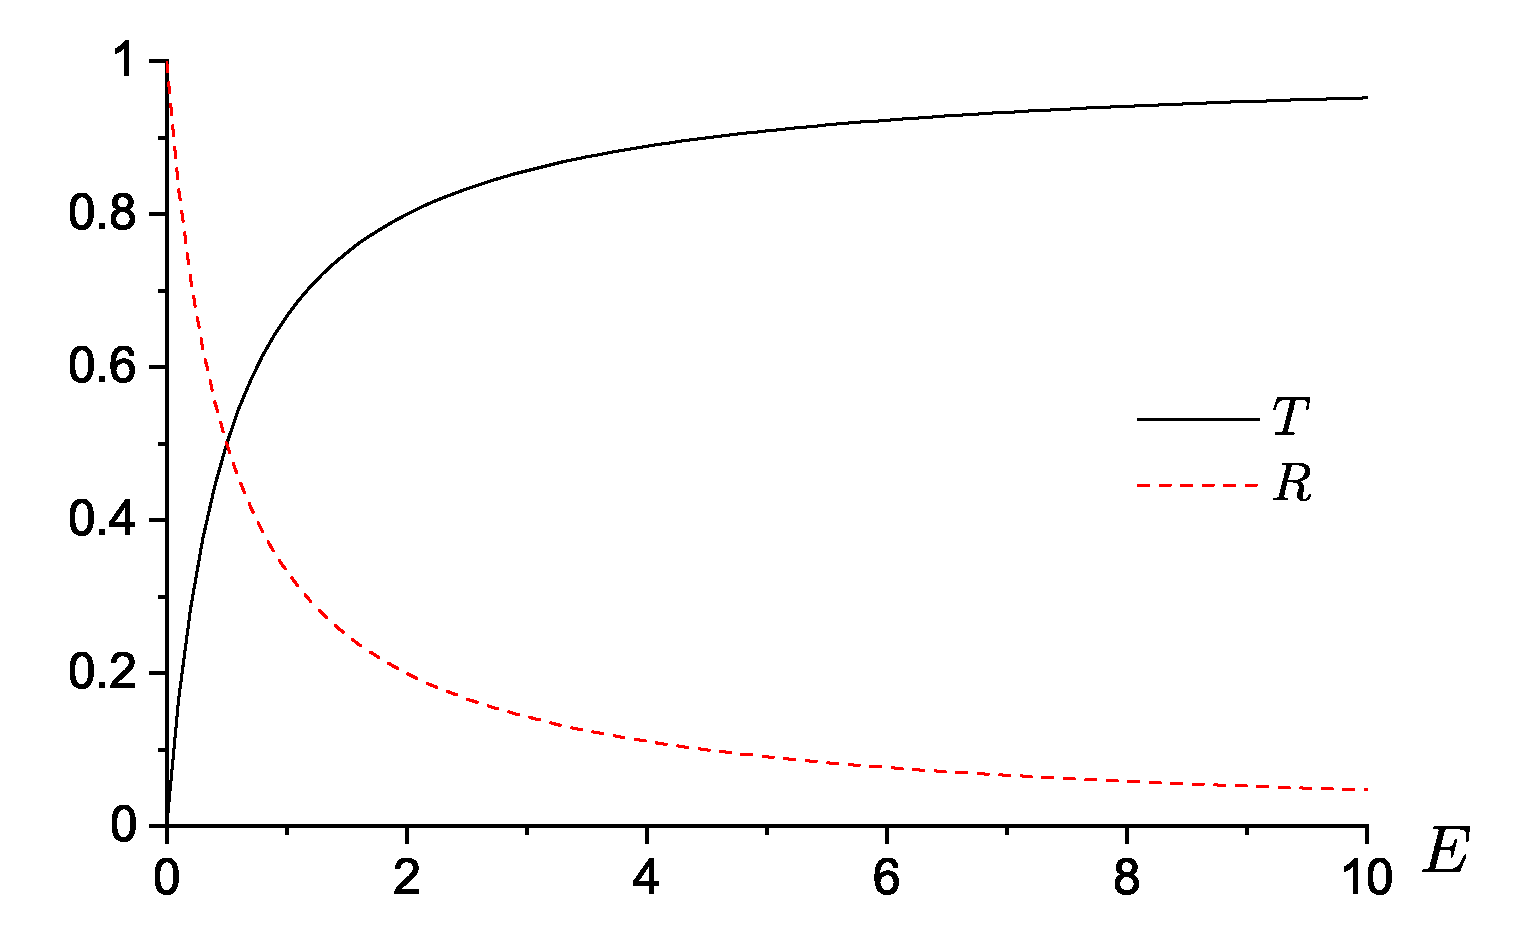
\epsfig{file=figures/deltatr.eps,width=0.6\linewidth}
			\scaption{
				Pravděpodobnost průchodu (černá čára) a odrazu (červená přerušovaná čára) pro potenciál tvořený jednou $\delta$ funkcí ($M=\hbar=c=1$).
                Jejich součet je roven 1.
			}
			\label{fig:DeltaTR}
		\end{figure}

		Sešívání vlnové funkce~\eqref{eq:DeltaBarrierWF} v bodě $x=0$ vede na podmínky
		\begin{subequations}
			\begin{align}
				A+B&=C,\\
				\im k(C+B-A)&=KC.
			\end{align}
		\end{subequations}
		Vyjádřením $B$ z první podmínky a dosazením do druhé se dostane
		\begin{equation}
			C=\frac{A}{1-\frac{K}{2ik}}.
		\end{equation}
		Pravděpodobnost průchodu je tedy
		\begin{equation}
			T=\frac{1}{1-\frac{K}{2ik}}\frac{1}{1+\frac{K}{2ik}}
			 =\frac{1}{1+\left(\frac{K}{2k}\right)^{2}}
			 =\frac{1}{1+\frac{Mc^{2}}{2\hbar^{2}E}}
			\label{eq:DeltaT}
		\end{equation}
		a analogicky pravděpodobnost odrazu
		\begin{equation}
			R=\frac{1}{1+\left(\frac{2K}{k}\right)^{2}}
			 =\frac{1}{1+\frac{2\hbar^{2}E}{Mc^{2}}}.
			\label{eq:DeltaR}
		\end{equation}
        Platí, že $T+R=1$. 
        Obě pravděpodobnosti jsou zakresleny na obrázku~\ref{fig:DeltaTR}.
        
        \begin{note}
            Povšiměte si, že $R$ ani $T$ nezávisejí na znaménku $c$, tj. pravděpodobnost průchodu a odrazu je při zadané energii stejná pro $\delta$ jámu i pro $\delta$ bariéru.
        \end{note}    
    					
	\item
		Fázové posunutí\sfootnote{
            Držíme se zavedené notace, proto pro fázové posunutí i pro $\delta$ funkci se používá stejné, přestože kolizní označení.} 
		$\delta$\index{posunutí!fázové} značí fázi, o kterou se posune rovinná vlna kvůli přítomnosti potenciálu oproti případu bez potenciálu.
		Situace je schematicky znázorněna na obrázku~\ref{fig:DeltaWFPhaseShift}.
		Pro určení fázového posunutí se vyjde z definice~\eqref{eq:PhaseShift}, což po dosazení dá
		\begin{equation}
			\delta=\arctan{\frac{\imaginary{\mathfrak{T}}}{\real{\mathfrak{T}}}}
				=-\arctan{\frac{K}{2k}}
				=-\arctan{c\sqrt{\frac{M}{2\hbar^{2}E}}}.
			\label{eq:DeltaPhaseShift}
		\end{equation}
		Energetická závislost fázového posunutí je zakreslena na obrázku~\ref{fig:DeltaPhaseShift}.

		\begin{figure}[!htbp]
			\centering
			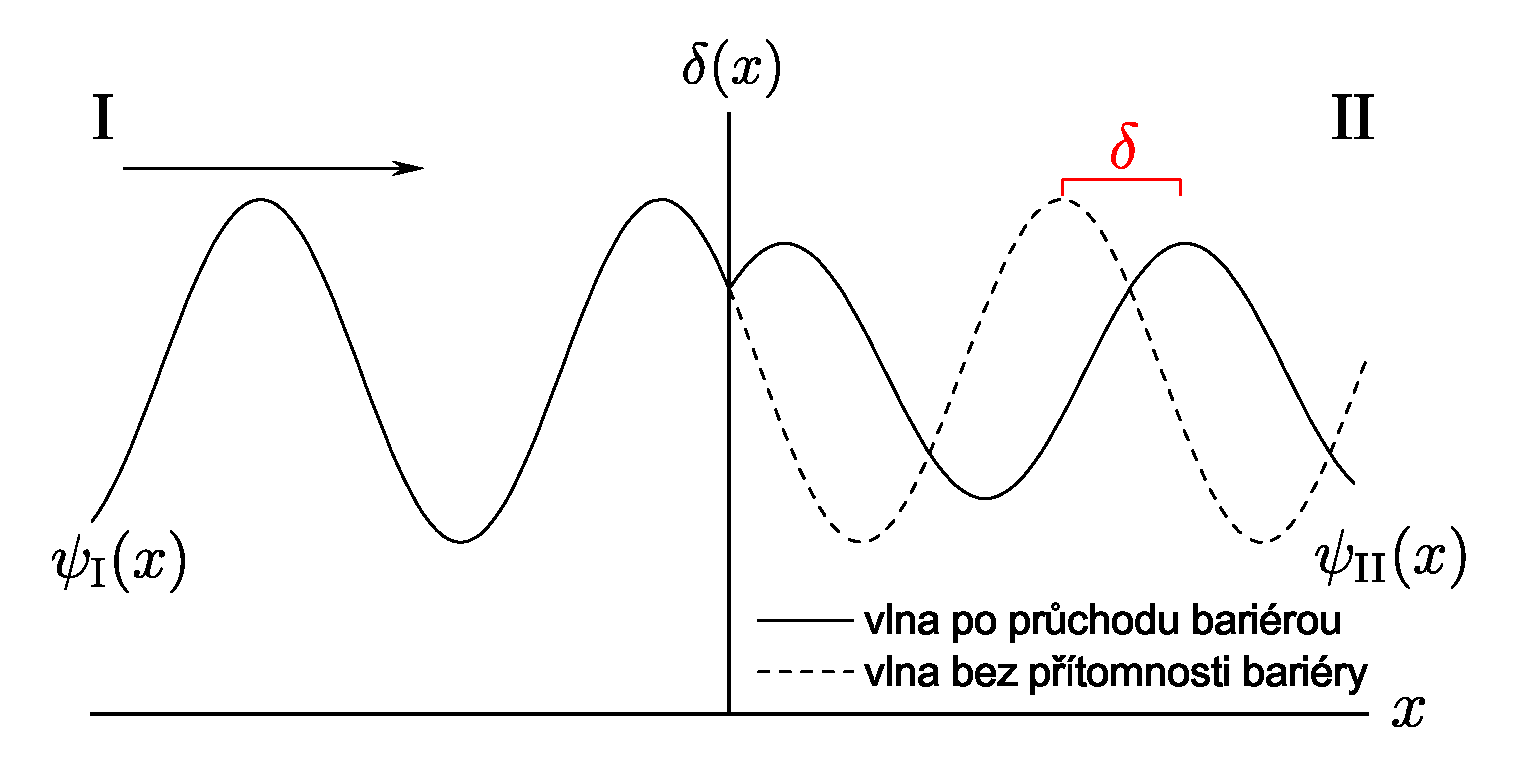
\epsfig{file=figures/deltasin.eps,width=0.7\linewidth}
			\scaption{
				Vlnová funkce pro výpočet fázového posunutí $\delta$ (červeně).
				Vlnová funkce za nepřítomnosti potenciálu $V(x)=c\,\delta(x)$ je znázorněna přerušovanou čarou.
			}
			\label{fig:DeltaWFPhaseShift}
		\end{figure}
		
		\begin{figure}[!htbp]
			\centering
			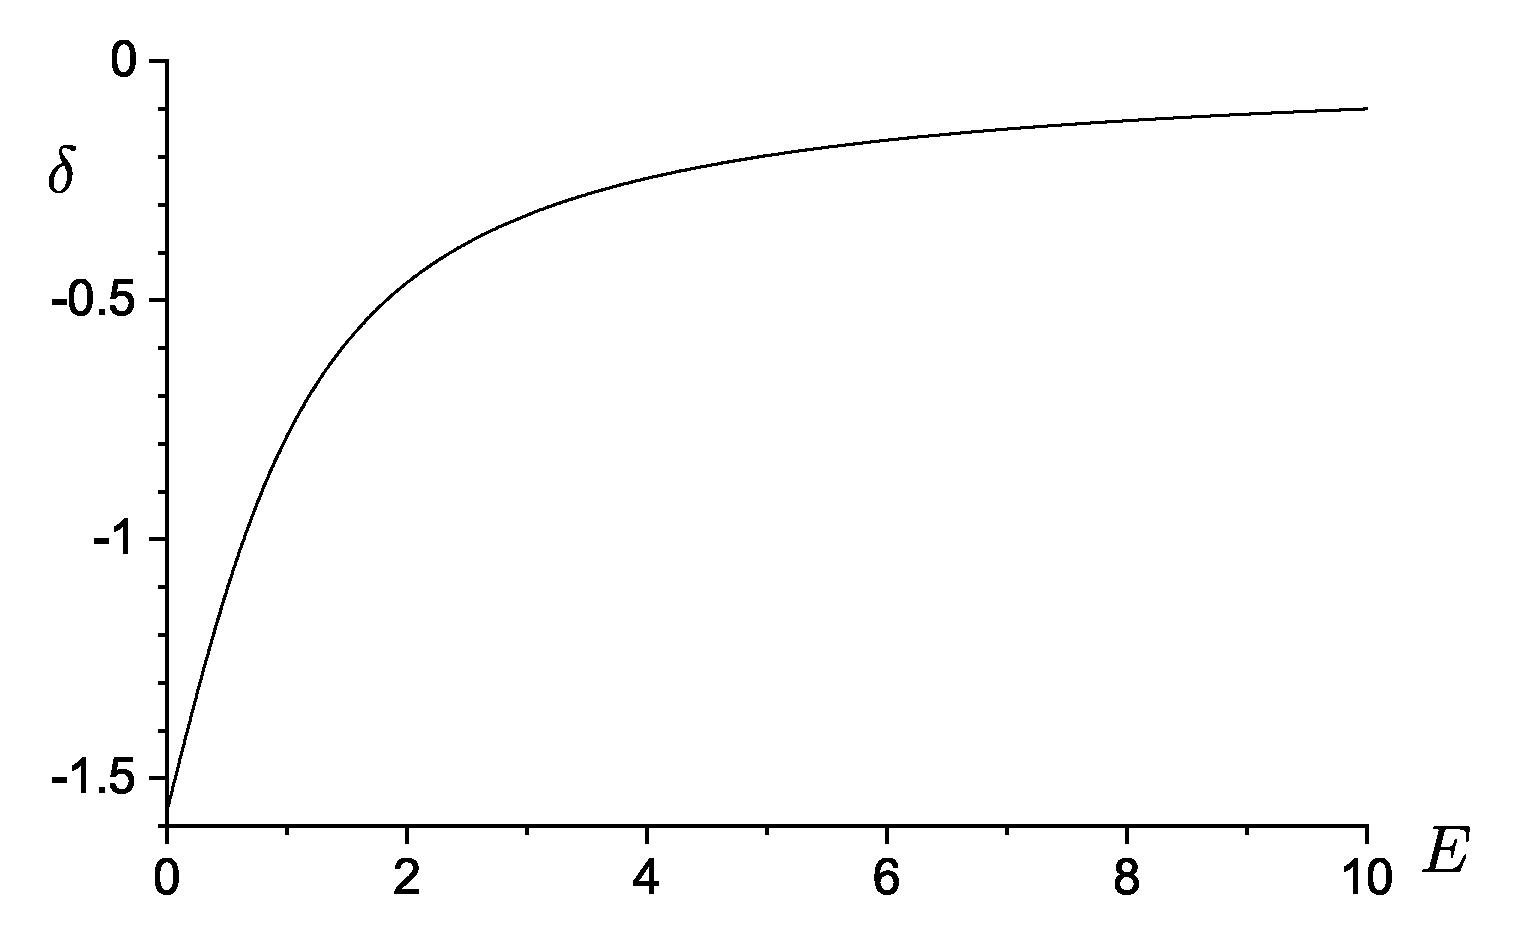
\epsfig{file=figures/deltadelta.eps,width=0.6\linewidth}
			\scaption{
				Fázové posunutí pro jednu $\delta$ funkci ($M=\hbar=c=1$).
			}
			\label{fig:DeltaPhaseShift}
		\end{figure}			
	\end{enumerate}	
\end{solution}

\begin{note}
    Potenciál ve tvaru $\delta$ funkce má simulovat velmi úzkou a hlubokou potenciálovou jámu, resp. bariéru.
    Jedná se vlastně o limitní případ konečné jámy (bariéry) šířky $a$ a hloubky (výšky) $v$, kde $a\rightarrow0$ a zároveň $va\equiv c=\const$.
\end{note}
